\section{CTST - Lớp 10 - Ôn tập giữa học kì 1 - Đề 6}
\caulc
\Opensolutionfile{ans}[ans-ABCD]

\begin{ex}%[0D1N1-3]
	Cho mệnh đề $A:~$\lq\lq $\forall x \in \mathbb{R}, x^2-x+7<0$\rq\rq. Mệnh đề phủ định của $A$ là
	\choice
	{$\forall x \in \mathbb{R}, x^2-x+7>0$}
	{$\forall x \in \mathbb{R}, x^2-x+7>0$}
	{Không tồn tại $x: x^2-x+7<0$}
	{\True$\exists x \in \mathbb{R}, x^2-x+7 \geq 0$}
	\loigiai{
	Mệnh đề phủ định của $A$ là \lq\lq $\exists x \in \mathbb{R}, x^2-x+7 \geq 0$\rq\rq.
	}
\end{ex}
\begin{ex}%[0D1H1-2]
	Mệnh đề nào sau đây là \textbf{sai}?
	\choice
	{$\exists x \in \mathbb{R}: x>x^2$}
	{$\exists n \in \mathbb{N}: n^2=n$}
	{$\forall n \in \mathbb{N}$ thì $n \leq 2n$}
	{\True $\forall x \in \mathbb{R}: x^2>0$}
	\loigiai{
	Khi $x=0$ thì mệnh đề này \lq\lq $\forall x \in \mathbb{R}: x^2>0$\rq\rq~ không đúng. 
	}
\end{ex}
\begin{ex}%[0D1H3-3]
	Cho tập hợp $A=[-2; 2]$, $B=(1; 5]$. Khi đó $A\cap B$ là
	\choice
	{$[-2; 5]$}
	{$\{0\}$}
	{$[1; 2)$}
	{\True $(1; 2]$}
	\loigiai{
	Ta có $A\cap B = (1; 2]$.}
\end{ex}
\begin{ex}%[0D1N3-1]
	Cho hai tập hợp: $X=\{1; 2; 3; 4; 5; 6\}$ và $Y=\{1; 4; 6; 7; 9\}$. Tính $X \cap Y$?
	\choice
	{$\{1; 2; 3; 4\}$}
	{$\{2; 3; 5; 7; 9\}$}
	{$\{1; 2; 3; 4; 5; 6; 7; 9\}$}
	{\True $\{1; 4; 6\}$}
	\loigiai{
	$X \cap Y=\{\forall x \mid x \in X, x \in Y\} \Rightarrow X \cap Y=\{1; 4; 6\}$.}
\end{ex}
\begin{ex}%[0D2H1-2]
	Miền nghiệm của bất phương trình $5(x+2)-9<2 x-2 y+7$ là phần mặt phẳng không chứa điểm nào?
	\choice
	{$(-2; 1)$}
	{\True $(2; 3)$}
	{$(2; -1)$}
	{$(0; 0)$}
	\loigiai{
	Cặp số $(2; 3)$ không thỏa bất phương trình.
	}
\end{ex}
\begin{ex}%[0D3N1-2]
	Tập xác định của hàm số $y=\dfrac{1}{x-3}$ là
	\choice
	{\True $\mathbb{R} \setminus\{3\}$}
	{$\mathbb{R} \setminus\{0\}$}
	{$(3 ;+\infty)$}
	{$\mathbb{R}$}
	\loigiai{Hàm số xác định $\Leftrightarrow x-3 \neq 0 \Leftrightarrow x \neq 3$.\\
	Vậy tập xác định của hàm số là $\mathbb{R} \setminus\{3\}$.}
\end{ex}
\begin{ex}%[0D3H2-2]
	Hàm số $y=-4x^2+16x+2025$ nghịch biến trên khoảng nào sau đây?
	\choice
	{\True$(2 ;+\infty)$}
	{$(-\infty ; 2)$}
	{$(-2 ;+\infty)$}
	{$(-\infty ;-2)$}
	\loigiai{
	Hàm số $y=-4x^2+ 16x+2025$ với hệ số $a=-4<0$ và $-\dfrac{b}{2a}=2$ cho nên hàm số nghịch biến trên khoảng $(2; +\infty)$.}
\end{ex}
\begin{ex}%[0D3N2-2]
	Hàm số $y=f(x)=ax^2+ bx+c ~(a \neq 0)$ có bảng biến thiên như sau
	\begin{center}
	
\begin{tikzpicture}
		\tkzTabInit[espcl=3.0,lgt=1.5,nocadre]
		{$x$/0.7,$f(x)$/2.1}
		{$-\infty$,$2$,$+\infty$}
		%\tkzTabLine{,-,0,+}
		\tkzTabVar{+/$+\infty$,-/$-1$,+/$+\infty$}
	\end{tikzpicture}
	\end{center}
	Hỏi hàm số đã cho đạt giá trị nhỏ nhất khi $x$ bằng bao nhiêu?	
	\choice
	{\True $2$}
	{$-1$}
	{$-2$}
	{$1$}
	\loigiai{Từ bảng biến thiên của hàm số ta thấy hàm số đạt giá trị nhỏ nhất bằng $-1$ khi $x=2$.}
\end{ex}
\begin{ex}%[0H4N1-2]
	 Giá trị của biểu thức $P=\cos 45^\circ \cdot \cos 60^\circ-\sin 45^\circ \cdot \sin 60^\circ$ là
	\choice
	{$P=\dfrac{-\sqrt{6}-\sqrt{2}}{2}$}
	{$P=\dfrac{-\sqrt{6}-\sqrt{2}}{4}$}
	{\True$P=\dfrac{-\sqrt{6}+\sqrt{2}}{4}$}
	{$P=\dfrac{-\sqrt{6}+\sqrt{2}}{2}$}
	\loigiai{
	Ta có $P=\cos 45^\circ \cdot \cos 60^\circ-\sin 45^\circ \cdot \sin 60^\circ=\dfrac{-\sqrt{6}+\sqrt{2}}{4}$.}
\end{ex}
\begin{ex}%[0H4H1-2]
	Cho góc $\alpha$ thỏa mãn $90^\circ<\alpha<180^\circ$ và $\sin \alpha=\dfrac{3}{4}$. Tính $\cos \alpha$.
	\choice
	{$-\dfrac{\sqrt{7}}{3}$}
	{$\dfrac{\sqrt{7}}{3}$}
	{\True$-\dfrac{\sqrt{7}}{4}$}
	{$\dfrac{\sqrt{7}}{4}$}
	\loigiai{Ta có $90^\circ<\alpha<180^\circ$ suy ra $\cos \alpha=-\sqrt{1-\sin^2\alpha}=-\sqrt{1-\dfrac{9}{16}}=-\dfrac{\sqrt{7}}{4}$.}
	
\end{ex}
\begin{ex}%[0D2H2-2]
	Phần không tô đậm trong hình vẽ dưới đây (không chứa biên) biểu diễn miền nghiệm của hệ bất phương trình nào trong các hệ bất phương trình sau?
	\begin{center}
	\begin{tikzpicture}[line join=round, line cap=round,>=stealth,thick]
		\tikzset{every node/.style={scale=0.9}}
		\begin{scope}
			\clip (-2.5,-2) rectangle (6,4);
			\fill[pattern=horizontal lines] (-3.5,4.33)--(-3.5,-2.67)--(7,-2.67)--cycle;
			\fill[pattern=horizontal lines] (-4.5,-2.12)--(21,-2.12)--(21,4.25)--cycle;
			\draw (-3,4)--(6,-2) node [pos=0.1, above, sloped] {$d_1$};
			\draw (6,0.5)--(-4,-2) node [pos=0.05, above, sloped] {$d_2$};
		\end{scope}
		\draw[->] (-2.5,0)--(6,0) node[below]{$x$};
		\draw[->] (0,-2)--(0,4) node[left]{$y$};
		\draw (0,0) node[below left]{$O$};
		\foreach \x in {3,4}
		\draw[thin] (\x,1pt)--(\x,-1pt) node [above] {$\x$};
		\foreach \y in {-1,2}
		\draw[thin] (1pt,\y)--(-1pt,\y) node [above right] {$\y$};
	\end{tikzpicture}
	\end{center}
	\choice
	{$\heva{&2x+3y \geq 6 \\& x-4y \leq 4}$}
	{$\heva{&2x+3y<6 \\& x-4 y>4}$}
	{$\heva{&2x+3y>6 \\& 4x-y<4}$}
	{\True$\heva{&2x+3y>6 \\& x-4 y<4}$}
	\loigiai{
	Từ hình vẽ, ta có đường thẳng $d_1$ đi qua hai điểm $A(0; 2)$; $B(3; 0)$ nên $d_1\colon 2x+3y=6$.\\
	Từ hình vẽ, ta có đường thẳng $d_2$ đi qua hai điểm $C(0; -1)$; $B(4 ; 0)$ nên $d_2\colon x-4y=4$.
	\begin{itemize}
	\item Vẽ đường thẳng $d_1\colon 2x+3y=6$, miền chứa điểm $O(0; 0)$ không phải là miền nghiệm nên khi thế tọa độ điểm $O(0;0)$ vào ta phải được bất phương trình sai, nghĩa là $0>6$. Vậy bất phương trình cần tìm là $2x+3y>6$.
	\item Vẽ đường thẳng $d_2\colon x-4y=4$, miền chứa điểm $O(0; 0)$  là miền nghiệm nên khi thế tọa độ điểm $O(0;0)$ vào ta phải được bất phương trình đúng, nghĩa là $0<4$. Vậy bất phương trình cần tìm là $x-4y<4$.
	\end{itemize}
}
\end{ex}
\begin{ex}%[0D3V2-1]
	Cho hàm số $y=f(x)=ax^2+bx+c$ có đồ thị như hình vẽ dưới đây
	\begin{center}
	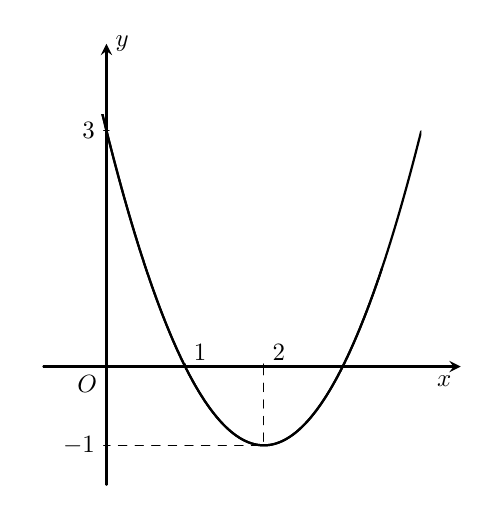
\begin{tikzpicture}[line join=round, line cap=round,>=stealth,thick]
		\tikzset{every node/.style={scale=0.9}}
		\draw[->] (-0.8,0)--(4.5,0) node[below left] {$x$};
		\draw[->] (0,-1.5)--(0,4.1) node[right] {$y$};
		\draw (0,0) node [below left] {$O$};
		\foreach \x/\nx in {1/1,2/2}
		\draw[thin] (\x,1pt)--(\x,-1pt) node [above right] {$\nx$};
		\foreach \y/\ny in {-1/-1,3/3}
		\draw[thin] (1pt,\y)--(-1pt,\y) node [left] {$\ny$};
		\draw[dashed,thin](2,0)--(2,-1)--(0,-1);
		\begin{scope}
			\clip (-1,-1.5) rectangle (4,3.2);
			\draw[samples=200,domain=-0.5:3.5,smooth,variable=\x] plot (\x,{1*(\x)^2+-4*(\x)+3});
			\draw[samples=200,domain=-0.5:4,smooth,variable=\x] plot (\x,{1*(\x)^2+-4*(\x)+3});
		\end{scope}
	\end{tikzpicture}
	\end{center}
	Tính $f(-1)$.
	\choice
	{$f(-1)=7$}
	{$f(-1)=0$}
	{\True$f(-1)=8$}
	{$f(-1)=9$}
	\loigiai{
	Ta có $\heva{&f(0)=3 \\& f(1)=0 \\& f(2)=-1} \Leftrightarrow\heva{&c=3 \\& a+b+c=0 \\& 4a+2b+c=-1} \Leftrightarrow\heva{&c=3 \\& a=1 \\& b=-4.}$\\
	Vậy $f(x)=x^2-4x+3 \Rightarrow f(-1)=8$.}
\end{ex}	
\Closesolutionfile{ans}

\indapan{6}{ans-ABCD}

\cauds

\Opensolutionfile{ans}[ans-DS]
\setcounter{ex}{0}
\begin{ex}%[0D1H3-5] 
	Lớp $10 C 6$ có $18$ học sinh tham gia câu lạc bộ bóng đá và $15$ học sinh tham gia câu lạc bộ bóng rổ. Biết rằng có $10$ học sinh tham gia cả hai câu lạc bộ trên. Khi đó:
\choiceTF
{\True Có $8$ học sinh tham gia câu lạc bộ bóng đá và không tham gia câu lạc bộ bóng rổ}
{\True Có $23$ học sinh tham gia ít nhất một trong hai câu lạc bộ trên}
{Biết lớp $10C6$ có $45$ học sinh. Có $25$ học sinh không tham gia câu lạc bộ bóng đá}
{ Biết lớp $10C6$ có $45$ học sinh. Có $24$ học sinh không tham gia cả hai câu lạc bộ}
\loigiai{
Kí hiệu: $A$ là tập hợp học sinh tham gia câu lạc bộ bóng đá, $B$ là tập hợp học sinh tham gia câu lạc bộ bóng rổ, $E$ là tập hợp học sinh của lớp $10C6$.\\
Ta có thể biểu diễn ba tập hợp trên bằng biểu đồ Ven như hình sau:
\begin{center}
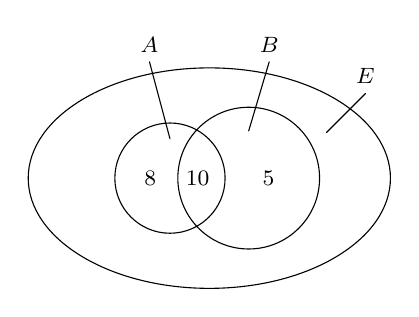
\begin{tikzpicture}[scale=1, font=\footnotesize, line join=round, line cap=round, >=stealth]
	\path 
	(0,0) coordinate (O)
	(O)+(-.5,0) coordinate (C)
	(O)+(.5,0) coordinate (E)
	(1.8,0) arc (0:30:1.8cm and 1.3cm) coordinate (B)
		;
	\draw (C) circle (0.7cm) (E) circle (.9cm);
	\draw (C)+(90:.5)--+(100:1.5) node[above]{$A$};
	\draw (E)+(90:.6)--+(80:1.5) node[above]{$B$};
	\draw (O) ellipse (2.3cm and 1.4cm);
	\draw (B)+(-135:.1)--+(45:.6) node[above]{$E$};
	\draw (-.15,0) node{$10$};
	\draw (-.75,0) node{$8$};
	\draw (.75,0) node{$5$};
\end{tikzpicture}
		\end{center}
Khi đó, $A \cap B$ là tập hợp học sinh tham gia cả hai câu lạc bộ trên. Số phần tử của $A$ là $18 $, số phần tử của $B$ là $15 $, số phần tử của tập hợp $A \cap B$ là $10 $.
\begin{itemchoice}
			\itemch \textbf{Đúng}.\\Tập hợp các học sinh tham gia câu lạc bộ bóng đá và không tham gia câu lạc bộ bóng rổ là tập hợp $A \setminus B$. Số phần tử của $A \setminus B$ chính là số phần tử của $A$ trừ đi số phần tử của $A \cap B$.\\ Vậy số học sinh tham gia câu lạc bộ bóng đá và không tham gia câu lạc bộ bóng rổ là $18-10=8$ (học sinh).
\itemch \textbf{Đúng}.\\Tập hợp các học sinh tham gia ít nhất một trong hai câu lạc bộ trên chính là tập hợp $A \cup B$. Do khi đếm số học sinh tham gia câu lạc bộ bóng đá là $18 $, số học sinh tham gia câu lạc bộ bóng rổ là $15$ thì số học sinh tham gia cả hai câu lạc bộ là $10$ được tính hai lần. Vậy số học sinh tham gia ít nhất một trong hai câu lạc bộ trên là $18+15-10=23$ (học sinh).
\itemch \textbf{Sai}.\\Số phần tử của $E$ là $45 $. Tập hợp các học sinh không tham gia câu lạc bộ bóng đá là phần bù của $A$ trong $E$. Vậy số học sinh không tham gia câu lạc bộ bóng đá là $45-18=27$ (học sinh). 
\itemch \textbf{Sai}.\\Tập hợp các học sinh không tham gia cả hai câu lạc bộ là phần bù của $A \cup B$ trong $E$. Vậy số học sinh không tham gia cả hai câu lạc bộ là $45-23=22$ (học sinh).
\end{itemchoice}
}
\end{ex}

\begin{ex}%[0D2V2-2]
Cho hệ bất phương trình $\heva{&3 x+2 y \geq 9 \\& x-2 y \leq 3 \\& x+y \leq 6 \\& x \geq 1}$ $(I)$. Các mệnh đề sau đúng hay \textbf{sai}?
\choiceTF
{ Miền nghiệm của hệ bất phương trình là miền tam giác}
{\True  $(3 ; 2)$ là một nghiệm của hệ bất phương trình}
{ $x=1$, $y=3$ là nghiệm của hệ bất phương trình $(I)$ sao cho $F=3 x-y$ đạt giá trị lớn nhất}
{\True  $x=1$, $ y=5$ là nghiệm của hệ bất phương trình $(I)$ sao cho $F=3 x-y$ đạt giá trị nhỏ nhất}
\loigiai{
\begin{itemchoice}
			\itemch \textbf{Sai}.\\Miền nghiệm của hệ $(I)$ là miền tứ giác $A B C D$ với $A(3 ; 0)$, $B(5 ; 1)$, $C(1 ; 5)$, $D(1 ; 3)$ (Hình vẽ dưới).
			\begin{center}
 \begin{tikzpicture}[scale=1, font=\footnotesize, line join=round, line cap=round, >=stealth]
 \def\xmin{-3}\def\xmax{7}\def\ymin{-2}\def\ymax{7}
\draw[->] (\xmin,0)--(\xmax,0) node[below]{$x$};
\draw[->] (0,\ymin)--(0,\ymax) node[right]{$y$};
 \foreach \x in {3,5,6}
 \draw[shift={(\x,0)},color=black] (0pt,2pt) -- (0pt,-2pt) node[below] {\footnotesize $\x$};
 \foreach \x in {1}
 \draw[shift={(\x,0)},color=black] (0pt,2pt) -- (0pt,-2pt) node[below left] {\footnotesize $\x$};
  \foreach \y in {1,3,6}
 \draw[shift={(0,\y)},color=black] (2pt,0pt) -- (-2pt,0pt) node[left] {\footnotesize $\y$};
 \foreach \y in {5}
 \draw[shift={(0,\y)},color=black] (-2pt,0pt) -- (2pt,0pt) node[right] {\footnotesize $\y$};
 \draw[step=1,gray,black!20!white!]
(\xmin,\ymin) grid (\xmax,\ymax);
 \clip (\xmin,\ymin) rectangle (\xmax,\ymax);

 \fill[pattern=north east lines] (13/3,-2) -- (\xmin,-2) -- (\xmin,\ymax) -- (-5/3,\ymax)-- cycle;
 \draw[thick,smooth,samples=200,domain=\xmin:\xmax] plot(\x,{(-1.5)*(\x)+4.5});
 
 \fill[pattern=crosshatch dots] (-1,-2)--(\xmax,-2)--(\xmax,2)-- cycle;
 \draw[thick,smooth,samples=200,domain=\xmin:\xmax] plot(\x,{.5*(\x)-1.5});
 
 \fill[pattern=north west lines] (-1,\ymax)--(\xmax,\ymax) --(\xmax,-1)-- cycle;
 \draw[thick,smooth,samples=200,domain=\xmin:\xmax] plot(\x,{(-1)*(\x)+6});
 \fill[pattern=north west lines] (-1,\ymax)--(\xmax,\ymax) --(\xmax,-1)-- cycle;
 
 \fill[pattern=north west lines] (1,\ymin)--(\xmin,\ymin) --(\xmin,\ymax)--(1,\ymax)-- cycle;
 \draw (1,\ymin)--(1,\ymax);
 \coordinate [label= above: $A$](A) at (3,0) ; 
 \coordinate [label= above: $B$](B) at (5,1) ; 
 \coordinate [label= above right: $C$](C) at (1,5) ; 
  \coordinate [label=  right: $D$](D) at (1,3) ; 
  \foreach \diem in {A,B,C,D}	\fill (\diem)circle(2pt);
 \end{tikzpicture}
 \end{center}
	\itemch \textbf{Đúng}. \\Vì  $(3 ; 2)$ là một nghiệm của hệ bất phương trình.			\itemch \textbf{Sai}. \\Vì  tính giá trị của $F=3 x-y$ tại các cặp số $(x ; y)$ là tọa độ của các đỉnh tứ giác $A B C D$, ta có bảng sau: 
	\begin{center}
	\begin{tabular}{|c|c|c|c|c|}
	\hline
	&$A(3 ; 0)$ &$B(5 ; 1)$& $C(1 ; 5)$& $D(1 ; 3)$\\
	\hline
	$F=3 x-y$&$9$ &$14$& $-2$& $0$\\
	\hline
	\end{tabular}
	\end{center}
Vậy $F$ đạt giá trị lớn nhất bằng $14$ tại $x=5$, $ y=1$.
\itemch \textbf{Đúng}.\\ Vì   $F$ đạt giá trị nhỏ nhất bằng $-2$ tại $x=1$, $y=5$.
\end{itemchoice}
}
\end{ex}
\begin{ex}%[0D3H1-5]
Cho hàm số $y=f(x)=\dfrac{x+2}{x-1}$ có đồ thị là $(C)$.
\choiceTF
{\True Hàm số $y=f(x)$ có tập xác định là $D=\mathbb{R} \setminus\{1\}$}
{Đồ thị $(C)$ cắt trục hoành tại điểm $A(1 ; 0)$}
{\True  Điểm $B(2 ; 4)$ thuộc đồ thị $(C)$}
{ Hàm số $y=f(x)$ đồng biến trên khoảng $(1 ;+\infty)$}
\loigiai{
\begin{itemchoice}
			\itemch \textbf{Đúng}.\\ Vì  điều kiện xác định của hàm số là $x-1 \neq 0\Leftrightarrow x \neq 1$. 
			\itemch \textbf{Sai}.\\ Vì  xét $y=0 \Leftrightarrow \dfrac{x+2}{x-1}=0 \Leftrightarrow x+2=0 \Leftrightarrow x=-2$. \\Suy ra đồ thị $(C)$ cắt trục hoành tại điểm $D(-2 ; 0)$. 
			\itemch \textbf{Đúng}.\\ Vì  thế $x=2$, $ y=4$ vào $y=f(x)=\dfrac{x+2}{x-1}$ ta được $4=\dfrac{2+2}{2-1}$ (thỏa). Suy ra điểm $B(2 ; 4)$ thuộc đồ thị $(C)$. 
			\itemch \textbf{Sai}.\\ Vì  với mọi $x_1$, $ x_2 \in(1 ;+\infty)$, $ x_1 \neq x_2$. Ta có $$f\left(x_{2}\right)-f\left(x_{1}\right)=\dfrac{x_{2}+2}{x_{2}-1}-\dfrac{x_{1}+2}{x_{1}-1}=\dfrac{-3\left(x_{2}-x_{1}\right)}{\left(x_{2}-1\right)\left(x_{1}-1\right)}.$$
Xét $$T=\dfrac{f\left(x_{2}\right)-f\left(x_{1}\right)}{x_{2}-x_{1}} \Rightarrow T=\dfrac{f\left(x_{2}\right)-f\left(x_{1}\right)}{x_{2}-x_{1}}=-\dfrac{3}{\left(x_{2}-1\right)\left(x_{1}-1\right)}.$$
Ta thấy với $x_1$, $ x_2 \in(1 ;+\infty)$ thì $$x_2-1>0,x_1-1>0 \Rightarrow T=-\dfrac{3}{\left(x_{2}-1\right)\left(x_{1}-1\right)}<0.$$
Vậy hàm số đã cho nghịch biến trên khoảng $(1 ;+\infty)$. 
\end{itemchoice}
}
\end{ex}

\begin{ex}%[0D3H2-1]
\immini{Cho hàm số bậc hai $y=f(x)=a x^2+b x+c $ $(a \neq 0)$ có đồ thị $(P)$ như hình bên.}{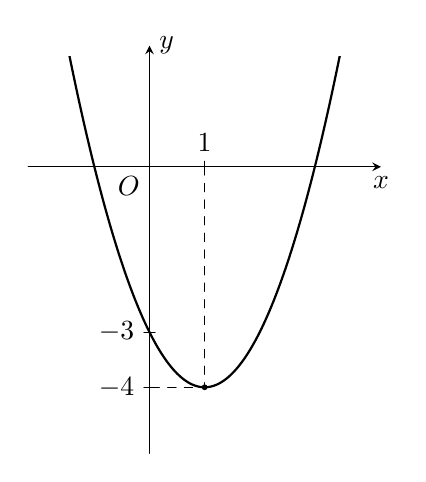
\begin{tikzpicture}[scale=0.7, line join=round, line cap=round, >=stealth]
\tikzset{every node/.style={scale=1}}
\def\xmin{-2}\def\xmax{4}\def\ymin{-5}\def\ymax{2}
\draw[->] (\xmin-0.2,0)--(\xmax+0.2,0) node[below]{$x$};
\draw[->] (0,\ymin-0.2)--(0,\ymax+0.2) node[right]{$y$};
\draw (0,0) node[below left]{$O$};
\foreach \x in {1}\draw (\x,-0.1)--(\x,0.1) node[above]{$\x$};
\foreach \y in {-4,-3}\draw (0.1,\y)--(-0.1,\y) node[left]{$\y$};
\clip (\xmin,\ymin) rectangle (\xmax,\ymax);
\draw[thick,smooth,samples=200,domain=\xmin:\xmax] plot (\x,{1*((\x)^2)+-2*\x+-3});
\draw[dashed] (1,0)--(1,-4)--(0,-4);\fill (1,-4)circle(1.5pt);
\end{tikzpicture}}
\choiceTF
{\True Đồ thị $(P)$ nhận đường thẳng $x=1$ làm trục đối xứng}
{\True  Hàm số $y=f(x)$ có bảng biến thiên là\\
\centerline{
\begin{tikzpicture}
\tkzTabInit[nocadre,lgt=1.2,espcl=2.5,deltacl=0.6]
{$x$/0.6,$y$/2}{$-\infty$,$1$,$+\infty$}
\tkzTabVar{+/$+\infty$,-/$-4$,+/$+\infty$}
\end{tikzpicture}}}
{ Giá trị lớn nhất của hàm số $y=f(x)$ trên đoạn $[0 ; 1]$ là $M=0$}
{\True  Hàm số đã cho có dạng $y=f(x)=x^2-2 x-3$}
\loigiai{
\begin{itemchoice}
			\itemch \textbf{Đúng}.\\ Vì  dựa vào đồ thị của hàm số ta có $x=1$ là trục đối xứng.
			\itemch \textbf{Đúng}.\\ Vì  dựa vào đồ thị của hàm số ta có đỉnh của $(P)$ là $I(1 ;-4)$ và $(P)$ có bề lõm hướng lên. Từ đó ta suy ra bảng biến thiên của hàm số. 
			\itemch \textbf{Sai}.\\ Vì  dựa vào đồ thị $(P)$ ta có giá trị lớn nhất của hàm số $y=f(x)$ trên đoạn $[0 ; 1]$ là $M=-3$. Đạt được khi $x=0$. 
			\itemch \textbf{Đúng}.\\ Vì  đồ thị $(P)$ của hàm số $y=f(x)$ có trục đối xứng là $x=1$, đi qua các điểm $A(0 ;-3)$ và $I(1 ;-4)$ nên ta có hệ phương trình$$\heva{&-4=a+b+c \\& -\dfrac{b}{2 a}=1 \\& -3=c} \Leftrightarrow\heva{&c=-3 \\& a+b=-1 \\& 2 a+b=0} \Leftrightarrow\heva{&c=-3 \\& a=1 \\& b=-2.}$$ Dẫn đến $y=f(x)=x^2-2 x-3$.
\end{itemchoice}}
\end{ex}

\Closesolutionfile{ans}
\indapan{4}{ans-DS}

\caukq

\Opensolutionfile{ans}[ans-KQ]
\setcounter{ex}{0}

\begin{ex}%[0D1V3-3]
 Cho khoảng $A=(1 ; m+10)$ và nửa khoảng $B=[2 m+5 ; 13)$ ($m$ là tham số). Gọi $S$ là tập hợp tất cả các số nguyên $m$ sao cho $A \cup B=(1 ; 13)$. Tính tổng bình phương các phần tử của tập hợp $S$.
\shortans{$15$}
\loigiai{
Điều kiện đối với $m$ để tồn tại khoảng $A$ và nửa khoảng $B$ là $$\heva{&m+10>1 \\& 2 m+5<13} \Leftrightarrow-9<m<4\,(*).$$
Khi đó$$A \cup B=(1 ; 13) \Leftrightarrow\heva{&2 m+5>1 \\& 2 m+5 \leq m+10 \\& m+10 \leq 13} \Leftrightarrow\heva{&m>-2 \\& m \leq 5 \\& m \leq 3} \Leftrightarrow-2<m \leq 3.$$
Kết hợp $(*)$, ta được $-2<m \leq 3$.\\
Vì $m \in \mathbb{Z}$ nên tập hợp các số nguyên $m$ thỏa mãn yêu cầu của bài toán là $$S=\{-1 ; 0 ; 1 ; 2 ; 3\}.$$
Vậy $(-1)^2+0^2+1^2+2^2+3^2=15$.}
\end{ex}

\begin{ex}%[0D2V2-3]
 Một công ty trong một đợt quảng cáo và bán khuyến mãi hàng hóa, cần thuê xe để chở ít nhất $140$ người và ít nhất $9$ tấn hàng. Nơi thuê chỉ có hai loại xe $A$ và $B$. Trong đó xe loại $A$ có 10 chiếc, xe loại $B$ có $9$ chiếc. Một chiếc xe loại $A$ cho thuê với giá $4$ triệu, loại $B$ giá $3$ triệu. Biết rằng xe $A$ chỉ chở tối đa $20$ người và $0{,}6$ tấn hàng. Xe $B$ chở tối đa $10$ người và $1{,}5$ tấn hàng. Để chi phí vận chuyển là thấp nhất, thì cần thuê $x$ xe loại $A$ và $y$ xe loại $B$. Tính $y^3-x^3$.
\shortans{$-61$}
\loigiai{
Gọi $x$ là số xe loại $A$ $(0 \leq x \leq 10 ; x \in \mathbb{N})$, $ y$ là số xe loại $B$ $(0 \leq y \leq 9 $; $y \in \mathbb{N})$. Khi đó tổng chi phí thuê xe là $T=4 x+3 y$ (triệu đồng).\\
Xe $A$ chở tối đa $20$ người, xe $B$ chở tối đa $10$ người nên tổng số người $2$ xe chở tối đa được là $20 x+10 y$ (người).\\
Xe $A$ chở được $0{,}6$ tấn hàng, xe $B$ chở được $1{,}5$ tấn hàng nên tổng lượng hàng $2$ xe chở được là $0{,}6 x+1{,}5 y$ (tấn).\\
Theo giả thiết, ta có $\heva{&0 \leq x \leq 10 \\& 0 \leq y \leq 9 \\ &20 x+10 y \geq 140 \\& 0{,}6 x+1{,}5 y \geq 9.}$\hfill $(*)$\\
Biểu diễn miền nghiệm của hệ bất phương trình $(*)$ là tứ giác $A B C D$ kể cả miền trong của tứ giác (như hình vẽ bên dưới).
\begin{center}
 \begin{tikzpicture}[scale=1, font=\footnotesize, line join=round, line cap=round, >=stealth]
 \def\xmin{-1}\def\xmax{11}\def\ymin{-1}\def\ymax{10}
\draw[step=1,gray,black!20!white!]
(\xmin,\ymin) grid (\xmax,\ymax);
\draw[->] (\xmin,0)--(\xmax,0) node[below]{$x$};
\draw[->] (0,\ymin)--(0,\ymax) node[right]{$y$};
 \foreach \x in {1,2,3,4,5,6,7,8,9}
 \draw[shift={(\x,0)},color=black] (0pt,2pt) -- (0pt,-2pt) node[below] {\footnotesize $\x$};
 \foreach \x in {10}
 \draw[shift={(\x,0)},color=black] (0pt,2pt) -- (0pt,-2pt) node[below right] {\footnotesize $\x$};
  \foreach \y in {1,2,3,4,5,6,7,8}
 \draw[shift={(0,\y)},color=black] (2pt,0pt) -- (-2pt,0pt) node[left] {\footnotesize $\y$};
 \foreach \y in {9}
 \draw[shift={(0,\y)},color=black] (2pt,0pt) -- (-2pt,0pt) node[above left] {\footnotesize $\y$};
 \clip (\xmin,\ymin) rectangle (\xmax,\ymax);

 \fill[pattern=north east lines] (2,\ymax) -- (\xmin,\ymax) -- (\xmin,\ymin) -- (7.5,\ymin)-- cycle;
 \draw[thick,smooth,samples=200,domain=\xmin:\xmax] plot(\x,{(-2)*(\x)+14});
 
 \fill[pattern=crosshatch dots] (\xmin,6.4)--(\xmin,\ymin)--(\xmax,\ymin)--(\xmax,1.6)-- cycle;
 \draw[thick,smooth,samples=200,domain=\xmin:\xmax] plot(\x,{(-(0.6)/(1.5))*(\x)+9/(1.5)});
% 
% \fill[pattern=north west lines] (-1,\ymax)--(\xmax,\ymax) --(\xmax,-1)-- cycle;
% \draw[thick,smooth,samples=200,domain=\xmin:\xmax] plot(\x,{(-1)*(\x)+6});
% \fill[pattern=north west lines] (-1,\ymax)--(\xmax,\ymax) --(\xmax,-1)-- cycle;
% 
 \fill[pattern=north west lines] (10,\ymin)--(\xmax,\ymin) --(\xmax,\ymax)--(10,\ymax)-- cycle;
 \draw (10,\ymin)--(10,\ymax);
 
 \fill[pattern=north west lines] (0,\ymin)--(\xmin,\ymin) --(\xmin,\ymax)--(0,\ymax)-- cycle;
 
 \fill[pattern=north west lines] (\xmin,9)--(\xmin,\ymax) --(\xmax,\ymax)--(\xmax,9)-- cycle;
 \draw (\xmin,9)--(\xmax,9);
 
 \fill[pattern=north west lines] (\xmin,0)--(\xmin,-1) --(\xmax,-1)--(\xmax,0)-- cycle;
 \coordinate [label= above right: $A$](A) at (10,2) ; 
 \coordinate [label= above right: $B$](B) at (10,9) ; 
 \coordinate [label= above right: $C$](C) at (2.5,9) ; 
  \coordinate [label= above right: $D$](D) at (5,4) ; 
  \foreach \diem in {A,B,C,D}	\fill (\diem)circle(2pt);
 \end{tikzpicture}
 \end{center}
Biểu thức $T=4 x+3 y$ đạt giá trị nhỏ nhất tại một trong các đỉnh của tứ giác $A B C D$.\\
Tại các đỉnh $A(10 ; 2) $; $ B(10 ; 9) $; $ C\left(\dfrac{5}{2} ; 9\right) ; $ $D(5 ; 4)$, ta có 
\begin{center}
	\begin{tabular}{|c|c|c|c|c|}
	\hline
	&$A(10 ; 2) $& $ B(10 ; 9) $& $ C\left(\dfrac{5}{2} ; 9\right) $& $D(5 ; 4)$\\
	\hline
	$T=4 x+3 y$&$46$ &$67$& $37$& $32$\\
	\hline
	\end{tabular}
	\end{center}
	Vậy $T$ đạt giá trị nhỏ nhất tại $x=5$, $y=4.$
Khi đó, $y^3-x^3=-61$.
}
\end{ex}

\begin{ex}%[0D2V2-3]
Bác Nam có $8$ ha đất dự định trồng hai loại hoa màu là đậu và cà chua. Biết rằng một ha trồng đậu cần $20$ công và lãi được $3$ triệu đồng, một ha trồng cà chua cần $30$ công và lãi được $4$ triệu đồng. Hỏi Bác Nam thu được tiền lãi cao nhất là bao nhiêu, biết tổng số công không quá $180$ công.\shortans{$26$}
\loigiai{
Gọi $x$, $ y$ lần lượt là số ha trồng đậu và trồng cà chua của hộ nông dân (Điều kiện $x$, $ y \geq 0$).\\
Số ngày công trồng đậu và cà chua của hộ nông dân là $20 x+30 y$.\\
Vì có tổng diện tích là $8$ ha trồng đậu và cà chua nên ta có bất phương trình $x+y \leq 8$.\\
Vì tổng số ngày công không vượt quá $180$ nên ta có bất phương trình $20 x+30 y \leq 180$ hay $2 x+3 y \leq 18$.\\
Khi đó ta có hệ bất phương trình $\heva{&x \geq 0 \\& y \geq 0 \\& x+y \leq 8 \\& 2 x+3 y \leq 18.}$\hfill$(1)$\\
Hệ bất phương trình có miền nghiệm là miền tứ giác $O A B C$ với $O(0 ; 0)$, $ A(0 ; 6), $ $B(6 ; 2)$ và $C(8 ; 0)$ (như hình vẽ bên dưới).
\begin{center}
 \begin{tikzpicture}[scale=1, font=\footnotesize, line join=round, line cap=round, >=stealth]
 \def\xmin{-1}\def\xmax{11}\def\ymin{-1}\def\ymax{10}
\draw[step=1,gray,black!20!white!]
(\xmin,\ymin) grid (\xmax,\ymax);
\draw[->] (\xmin,0)--(\xmax,0) node[below]{$x$};
\draw[->] (0,\ymin)--(0,\ymax) node[right]{$y$};
 \foreach \x in {1,2,3,4,5,6,7,8,9}
 \draw[shift={(\x,0)},color=black] (0pt,2pt) -- (0pt,-2pt) node[below] {\footnotesize $\x$};
 \foreach \x in {10}
 \draw[shift={(\x,0)},color=black] (0pt,2pt) -- (0pt,-2pt) node[below right] {\footnotesize $\x$};
  \foreach \y in {1,2,3,4,5,6,7,8}
 \draw[shift={(0,\y)},color=black] (2pt,0pt) -- (-2pt,0pt) node[left] {\footnotesize $\y$};
 \foreach \y in {9}
 \draw[shift={(0,\y)},color=black] (2pt,0pt) -- (-2pt,0pt) node[above left] {\footnotesize $\y$};
 \clip (\xmin,\ymin) rectangle (\xmax,\ymax);

 \fill[pattern=north east lines] (\xmin,9) -- (\xmin,\ymax) -- (\xmax,\ymax) -- (\xmax,\ymin)-- (9,\ymin)-- cycle;
 \draw[thick,smooth,samples=200,domain=\xmin:\xmax] plot(\x,{(-1)*(\x)+8});
 
 \fill[pattern=crosshatch dots] (\xmin,20/3)--(\xmin,\ymax)--(\xmax,\ymax)--(\xmax,\ymin)--(21/2,\ymin)-- cycle;
 \draw[thick,smooth,samples=200,domain=\xmin:\xmax] plot(\x,{(-(2)/(3))*(\x)+6});
\fill[pattern=north west lines] (0,\ymin)--(\xmin,\ymin) --(\xmin,\ymax)--(0,\ymax)-- cycle;
\fill[pattern=north west lines] (\xmin,0)--(\xmin,\ymin) --(\xmax,\ymin)--(\xmax,0)-- cycle;
% 
% \fill[pattern=north west lines] (\xmin,9)--(\xmin,\ymax) --(\xmax,\ymax)--(\xmax,9)-- cycle;
% \draw (\xmin,9)--(\xmax,9);
% 
% \fill[pattern=north west lines] (\xmin,0)--(\xmin,-1) --(\xmax,-1)--(\xmax,0)-- cycle;
 \coordinate [label= above right: $A$](A) at (0,6) ; 
 \coordinate [label= above right: $B$](B) at (6,2) ; 
 \coordinate [label= above: $C$](C) at (8,0) ; 
  \foreach \diem in {A,B,C}	\fill (\diem)circle(2pt);
 \end{tikzpicture}
 \end{center}
Tiền lãi $F(x, y)=3 x+4 y$ (triệu đồng)\\
Bài toán trở về bài toán tìm $x$, $ y$ thỏa mãn $(1)$ sao cho $F(x, y)$ lớn nhất và xảy ra tại một trong các điểm $O$, $ A$, $ B$, $ C.$\\
Ta thấy $F(0 ; 0)=0$, $ F(0 ; 6)=24$, $ F(6 ; 2)=26$ và $F(8 ; 0)=24$.\\
Tại điểm $B$ thì $F(x, y)$ đạt giá trị lớn nhất. Do đó cần trồng $6$ sào đậu và $2$ sào cà chua.\\
Hay ta có $x=6 $; $ y=2 \Rightarrow F=3\cdot 6+4\cdot 2=26$ (triệu đồng).}
\end{ex}

\begin{ex}%[0D3H1-7]
Một người khách đi taxi $4$ chỗ của một hãng hết $562\,000$ đồng. Tính số km đi được biết giá tiền được tính theo bảng sau:
\begin{center}
\begin{tabular}{|l|c|c|c|}
\hline
 & Giá mở cửa $(\mathbf{0 {,} 5} \mathbf{~ k m})$ & \begin{tabular}{c}
Giá cước các \\
kilômét tiếp theo \\
\end{tabular} & \begin{tabular}{c}
Giá cước từ \\
kilômét thứ $31$ \\
\end{tabular} \\
\hline
Taxi $4$ chỗ & $11\,000$ dồng & $14\,500$ đồng & $11\,600$ đồng \\
\hline
\end{tabular}
\end{center}
\shortans{$40{,}5$}
\loigiai{
Giá mở cửa hết $11\,000$ (đồng).\\
Đi $30$ km tiếp theo hết $14\,500 \cdot 30=435\,000$ (đồng).\\
Đi từ km $31$ đến km $40$ hết $11\,600 \cdot 10=116\,000$ (đồng).\\
Tổng số tiền là $11\,000+435\,000+116\,000=562\,000$ (đồng).\\
Quãng đường đã đi là $0{,}5+30+10=40{,}5~(\mathrm{km})$.}
\end{ex}

\begin{ex}%[0D3H2-1]
Biết đồ thị hàm số $y=x^2+b x+c$ đi qua hai điểm $M(1 ; 0), $ $N(-1 ;-4)$. Tính giá trị biểu thức $A=b+c$.
\shortans{$-1$}
\loigiai{
Hai điểm $M(1 ; 0)$, $ N(-1 ;-4)$ thuộc đồ thị hàm số nên ta có hệ
$$\heva{&1^2+b+c=0 \\& (-1)^2-b+c=-4} \Leftrightarrow\heva{&b+c=-1 \\& -b+c=-5} \Leftrightarrow\heva{&b=2 \\& c=-3.}$$
Vậy $A=b+c=-1$.
}
\end{ex}
\begin{ex}%[0H4H3-1]
\immini{Từ một tấm bìa hình tròn, bạn An cắt ra một hình tam giác có cạnh $A B=8$ cm, $ A C=13$ cm và góc $\widehat{B}=60^\circ$ (như hình vẽ bên). Xác định độ dài cạnh $B C$ (làm tròn kết quả đến hàng phần mười theo đơn vị xăng-ti-met).
\shortans{$15$}}{\begin{tikzpicture}[scale=.7]
\coordinate [label=below left:$B$](B) at (0,0);
	\coordinate [label=above:$A$](A) at (2.37,4.1);
	\coordinate [label=below right:$C$](C) at (6,0);
\coordinate (I) at (3,1);
\foreach \diem in {A,B,C,I}	\fill (\diem)circle(1.5pt);		
\pgfmathsetmacro\a{sqrt(10)}
\draw[smooth](A)--(B)--(C)--(A);
 \draw (I) circle (\a);
 \draw pic[draw, angle radius=4mm]{angle=C--B--A};
 \draw (1.75,.85) node[below left]{$60^\circ$};
 \draw ($(A)! .5 ! (B)$) node[above,rotate=60]{$8$ cm};
 \draw ($(A)! .5 ! (C)$) node[above,rotate=310]{$13$ cm};
		\end{tikzpicture}}
\loigiai{
Đặt $B C=x~(\mathrm{cm})$ $(x>0)$.\\
Áp dụng định lí côsin ta có $A C^2=A B^2+B C^2-2 A B \cdot B C \cdot \cos B$\\
Suy ra $13^2=8^2+x^2-2 \cdot 8 \cdot x \cdot \cos 60^\circ \Leftrightarrow x^2-8 x-105=0$.\\
Giải phương trình trên ta được $x=15$ hoặc $x=-7$. \\Vì $x>0$ nên $x=15$.
Vậy $B C=15~(\mathrm{cm})$.
}
\end{ex}

\Closesolutionfile{ans}
\indapan{6}{ans-KQ}

